\documentclass[tikz,border=4pt]{standalone}
\usepackage{tikz}
\usetikzlibrary{positioning,shapes.geometric,arrows.meta,fit,calc,backgrounds}

\definecolor{ctrlFill}{HTML}{dae8fc}
\definecolor{ctrlStroke}{HTML}{6c8ebf}
\definecolor{calcFill}{HTML}{cce5ff}
\definecolor{calcStroke}{HTML}{4a86e8}
\definecolor{dataFill}{HTML}{d5e8d4}
\definecolor{dataStroke}{HTML}{82b366}
\definecolor{newStroke}{HTML}{b85450}
\definecolor{pkrnCol}{HTML}{c44b3a}
\definecolor{hubFill}{HTML}{f8cecc}
\definecolor{hubStroke}{HTML}{b85450}
\definecolor{xfFill}{HTML}{fff2cc}
\definecolor{xfStroke}{HTML}{d6b656}

\begin{document}
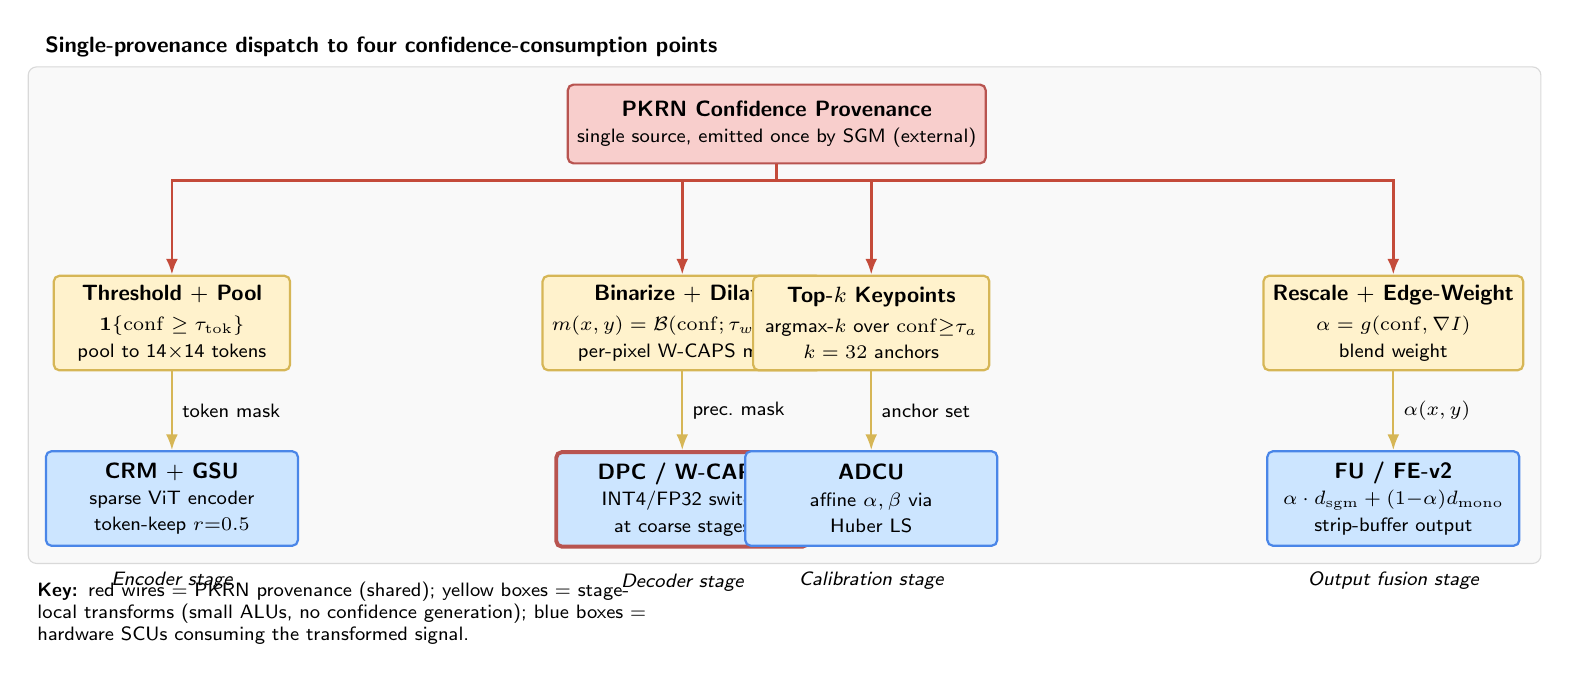
\begin{tikzpicture}[
  font=\footnotesize\sffamily,
  node distance=3mm,
  src/.style={draw=hubStroke, fill=hubFill, thick, minimum width=32mm, minimum height=10mm, align=center, rounded corners=2pt},
  xform/.style={draw=xfStroke, fill=xfFill, thick, minimum width=30mm, minimum height=12mm, align=center, rounded corners=2pt, font=\footnotesize\sffamily},
  scu/.style={draw=calcStroke, fill=calcFill, rounded corners=2pt, thick, minimum width=32mm, minimum height=12mm, align=center, inner sep=2pt},
  newscu/.style={draw=newStroke, fill=calcFill, rounded corners=2pt, line width=0.5mm, minimum width=32mm, minimum height=12mm, align=center, inner sep=2pt},
  pkrnarr/.style={-{Latex[length=2mm]}, thick, draw=pkrnCol, line width=0.35mm},
  derived/.style={-{Latex[length=2mm]}, thick, draw=xfStroke},
  datarr/.style={-{Latex[length=2mm]}, thick, draw=dataStroke},
  plbl/.style={font=\scriptsize\sffamily, text=pkrnCol, inner sep=1pt},
  math/.style={font=\scriptsize\sffamily}
]

% ============================================================
% SOURCE: single PKRN confidence provenance
% ============================================================
\node[src] (prov) at (0,0) {\textbf{PKRN Confidence Provenance}\\\scriptsize single source, emitted once by SGM (external)};

% ============================================================
% 4 LOCAL TRANSFORMS (row below source)
% ============================================================
\node[xform, below left=14mm and 35mm of prov] (xf1) {\textbf{Threshold $+$ Pool}\\[0.5mm]\scriptsize $\mathbf{1}\{\mathrm{conf} \geq \tau_{\mathrm{tok}}\}$\\\scriptsize pool to 14$\times$14 tokens};
\node[xform, below=14mm of prov, xshift=-12mm] (xf2) {\textbf{Binarize $+$ Dilate}\\[0.5mm]\scriptsize $m(x,y)=\mathcal{B}(\mathrm{conf}; \tau_{w}, 3{\times}3)$\\\scriptsize per-pixel W-CAPS mask};
\node[xform, below=14mm of prov, xshift=12mm] (xf3) {\textbf{Top-$k$ Keypoints}\\[0.5mm]\scriptsize argmax-$k$ over $\mathrm{conf}{\ge}\tau_a$\\\scriptsize $k=32$ anchors};
\node[xform, below right=14mm and 35mm of prov] (xf4) {\textbf{Rescale $+$ Edge-Weight}\\[0.5mm]\scriptsize $\alpha = g(\mathrm{conf}, \nabla I)$\\\scriptsize blend weight};

% ============================================================
% 4 SCU destinations (row below transforms)
% ============================================================
\node[scu, below=10mm of xf1] (crm) {\textbf{CRM $+$ GSU}\\\scriptsize sparse ViT encoder\\\scriptsize token-keep $r{=}0.5$};
\node[newscu, below=10mm of xf2] (dpc) {\textbf{DPC / W-CAPS}\\\scriptsize INT4/FP32 switch\\\scriptsize at coarse stages};
\node[scu, below=10mm of xf3] (adcu) {\textbf{ADCU}\\\scriptsize affine $\alpha,\beta$ via\\\scriptsize Huber LS};
\node[scu, below=10mm of xf4] (fu) {\textbf{FU / FE-v2}\\\scriptsize $\alpha\cdot d_{\mathrm{sgm}} + (1{-}\alpha)d_{\mathrm{mono}}$\\\scriptsize strip-buffer output};

% ============================================================
% RED confidence wires: prov -> each transform
% ============================================================
\draw[pkrnarr] (prov.south) -- ++(0,-2mm) -| (xf1.north);
\draw[pkrnarr] (prov.south) -- ++(0,-2mm) -| (xf2.north);
\draw[pkrnarr] (prov.south) -- ++(0,-2mm) -| (xf3.north);
\draw[pkrnarr] (prov.south) -- ++(0,-2mm) -| (xf4.north);

% ============================================================
% YELLOW (derived) arrows: transforms -> SCU destinations
% ============================================================
\draw[derived] (xf1.south) -- node[right, math]{token mask} (crm.north);
\draw[derived] (xf2.south) -- node[right, math]{prec.\ mask} (dpc.north);
\draw[derived] (xf3.south) -- node[right, math]{anchor set} (adcu.north);
\draw[derived] (xf4.south) -- node[right, math]{$\alpha(x,y)$} (fu.north);

% ============================================================
% PIPELINE-STAGE BAND ANNOTATIONS (below SCUs)
% ============================================================
\node[below=2mm of crm, font=\scriptsize\sffamily\itshape] {Encoder stage};
\node[below=2mm of dpc, font=\scriptsize\sffamily\itshape] {Decoder stage};
\node[below=2mm of adcu, font=\scriptsize\sffamily\itshape] {Calibration stage};
\node[below=2mm of fu, font=\scriptsize\sffamily\itshape] {Output fusion stage};

% ============================================================
% OUTER BOX + TITLE
% ============================================================
\begin{pgfonlayer}{background}
  \node[fit=(prov)(xf1)(xf4)(crm)(fu), fill=gray!5, rounded corners=3pt, inner sep=6pt, draw=gray!30] (outer) {};
\end{pgfonlayer}
\node[anchor=south west, font=\footnotesize\sffamily\bfseries] at ($(outer.north west)+(1mm,0mm)$) {Single-provenance dispatch to four confidence-consumption points};

% ============================================================
% LEGEND / NOTE
% ============================================================
\node[font=\scriptsize\sffamily, anchor=north west, text width=80mm] (note)
  at ($(outer.south west)+(0mm,-1mm)$)
  {\textbf{Key:} red wires = PKRN provenance (shared); yellow boxes = stage-local transforms (small ALUs, no confidence generation); \mbox{blue} boxes = hardware SCUs consuming the transformed signal.};

\end{tikzpicture}
\end{document}
